\section{Ergonomie}

	Nous avons également prévu d'implémenter des fonctionnalités plus secondaires, destinées à rendre \glasir{} suffisamment ergonomique pour être utilisé avec confort. Ces fonctionnalités n'apporteront pas de nouveautés en terme d'analyse, mais permettront de faciliter la manipulation des arbres et de rendre \glasir{} simple d'utilisation.	


	\subsection{Ouverture simultanée de plusieurs arbres}
		Dans sa version actuelle, ADTool ne permet de travailler que sur un seul arbre à la fois. Cette limitation est assez handicapante : par exemple, l'utilisateur ne peut pas ouvrir deux arbres en même temps pour les comparer. \glasir{} permettra donc d'ouvrir plusieurs instances d'ADTool, chacune contenant un arbre. Ces différentes instances se regrouperont sous la forme d'onglets situés dans l'interface de \glasir{}.
	
	\subsection{Hiérarchie des arbres}
		L'ouverture simultanée de plusieurs arbres induit la possibilité de manipuler un grand nombre d'arbres dans le cadre d'un même projet. \glasir{} fournira donc, dans un dock latéral, une arborescence de dossiers et de sous-dossiers contenant les différents arbres utilisés : l'utilisateur pourra ainsi facilement structurer la hiérarchie de son projet.
	
	\subsection{Bibliothèque de modèles}
		Il n'est pas forcément facile pour l'utilisateur de créer un arbre à partir de rien. C'est pourquoi \glasir{} fournira une bibliothèque d'arbres génériqes, aidant ainsi l'expert à démarrer son projet. Cette bibliothèque de modèles sera dupliquée pour être propre à chaque nouveau projet, permettant ainsi à l'utilisateur de modifier, compléter ou élaguer les arbres selon ses besoins.
		
		Si l'utilisateur construit un nouvel arbre qu'il juge pertinent de réutiliser dans un autre projet, il pourra enregistrer cet arbre comme nouveau modèle, qui se rajoutera donc à la bibliothèque. \glasir{} verra ainsi sa bibliothèque de modèles s'étoffer progressivement au cours du temps.

	
	\subsection{Couper/copier/coller}	
		Actuellement, ADTool ne permet pas l'utilisation des fonctions \emph{couper}/\emph{copier}/\emph{coller}, qui pourraient pourtant s'avérer pratiques lors de la création d'un arbre. Par exemple, dans le cas de l'oubli d'un nœud père, l'instauration de ces fonctionnalités permettrait de déplacer facilement les fils concernés de l'ancien nœud père vers le nouveau.
		
		En conséquence, nous allons modifier ADTool pour qu'il implémente ces fonctionnalités. Ainsi, la sélection d'un nœud entraînera la sélection de ses fils, afin de pouvoir couper ou copier ces nœuds facilement. Les raccourcis clavier \og classiques \fg{}  de ces fonctions (\emph{CTRL+X, CTRL+C, CTRL+V}) seront mis en place.

		Cependant, le \emph{copier} entraîne des questions de cohérence. En effet, si un arbre contient des nœuds avec le même label, il existe un moyen de simplifier l'arbre. Il faudra donc gérer ce cas de figure, à l'aide d'un message d'avertissement par exemple.

	\subsection{Amélioration du codage des arbres}
		ADTool affiche actuellement dans son interface une section nommée \emph{ADTerm Edit}. Celle-ci contient une représentation de l'arbre sous un format texte, en utilisant un langage propre au logiciel. Lors de la modification de l'arbre dans l'éditeur graphique, ADTool met à jour le texte correspondant en temps réel et de manière automatique. L'inverse est également vrai : il est possible de changer les labels des nœuds, ou les opérateurs, directement depuis \emph{ADTerm Edit} afin d'afficher ensuite le résultat graphiquement.

		Mais le langage qui permet de décrire les arbres sous format texte n'est pas très lisible : il ne contient par exemple pas le nom des nœuds autres que les feuilles. Sur la {\sc Figure} \ref{fig:int_adTool}, on peut constater que le code indique le nom des deux feuilles \og Acheter le matériel nécessaire \fg{} et \og Essayer les clés possibles \fg{}, et que la conjonction est bien précisée par l'opérateur \og ap \fg{} (\og op \fg{} en cas de disjonction). Mais aucune référence n'est faite au label du nœud père \og Casser le chiffrage \fg{}. Nous modifierons la grammaire pour corriger ce défaut, afin de rendre l'utilisation de cette fenêtre plus intuitive.

		\begin{figure}[h]
			\centering
			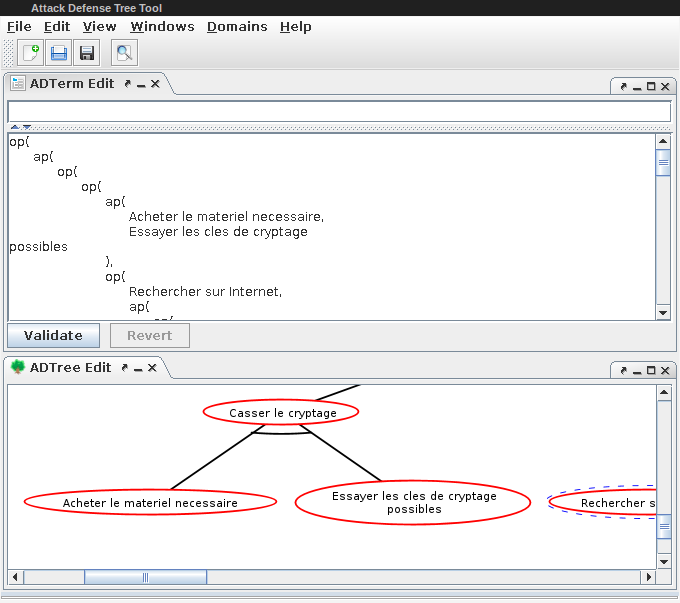
\includegraphics[width=0.6\textwidth]{figure/interface_adtool.png}
			\caption{L'interface d'ADTool. En haut, l'arbre au format texte ; en bas, sa représentation graphique.}
			\label{fig:int_adTool}
		\end{figure}
	
	\subsection{Annulation d'une action}	
		Pour le moment, effectuer une action sous ADTool est irréversible. Cela n'est pas grave pour certaines actions rapides à effectuer, telles que le renommage d'un nœud. Mais supprimer un nœud (ce qui implique la disparition de tous ses nœuds fils s'il y en a) par erreur peut entraîner un travail énorme, et donc une perte de temps. La possibilité de revenir à l'état précédent de l'arbre (par le raccourci clavier classique \emph{CTRL+Z}) éviterait d'avoir à refaire ce travail de construction fastidieux. Nous souhaitons créer au moins une sauvegarde de l'état précédent, afin de pouvoir annuler la dernière modification effectuée. Si possible, nous envisageons l'implémentation d'une pile circulaire contenant les N derniers états (chaque modification entraînant la création d'un nouvel état) avec un curseur pointant sur l'état courant. Cela permettrait de revenir en arrière sans contraintes. % préciser qu'on garde les modif et pas les états (sinon pb mémoires)

	\subsection{Vue globale des paramètres}
		Dans l'état actuel d'ADTool, lorsqu'un arbre est valué, un seul paramètre est affiché (le même pour tous les nœuds) même si plusieurs paramètres sont utilisés en réalité. En effet, chaque valuation a un onglet propre, dans lequel elle est la seule effectivement affichée sur l'arbre.% confus.
		Nous souhaitons créer un onglet plus général, dans lequel tous les paramètres voulus peuvent être visibles sur l'arbre en simultané. C'est ensuite à l'expert de décider des paramètres qu'il juge utile d'afficher. Cela serait aussi valable pour les paramètres de synthèse évoqués précédemment.\\
	
		Pour une meilleure lisibilité, chaque paramètre aura une couleur différente, et l'arbre sera accompagné d'une légende résumant ce jeu de coloration et ses correspondances. Nous devrons également gérer la taille des nœuds, pour que les paramètres ne dépassent pas de la bulle. Un tel système étant déjà présent dans ADTool pour gérer les labels, il suffira de l'étendre à l'affichage des paramètres.
